\chapter{Implementation}\label{Implementation}

In order to evaluate the effectiveness of the solution presented in Chapter~\ref{Design}, an implementation is developed using commonplace software and tools. This chapter outlines the steps taken to simulate a working prototype of the design in a virtual environment where metrics can be recorded inside reproducible scenarios. The project work produced as a result of this effort has been shared for your convenience and can be found in Appendix~\ref{project-files}.

In this chapter, the process for establishing a deterministic, configurable and measurable network evaluation environment using DebVM and QEMU is demonstrated. This is followed by an explanation and discussion of how BIND9 and NGINX are configured to realise the distributed deployment of ECH. Additionally, various traffic obfuscation techniques are instated using a combination of wireguard, tc and tcpdump. Finally, curl, Mozilla Firefox and Google Chrome are configured with ECH-support and shown to work with distributed ECH deployment.








\section{Simulation}

The initial time investment placed into a script for quick and configurable virtual testing environments was paramount for saving significant time and stress during the later iterative development process used to refine the design of the solution. The ability to teardown and setup a fresh virtual environment containing the exact same configuration in under a minute was vital during periods of investigation and debugging as well as evaluation and data collection. These virtual environments consist of many virtual machines connected together using a bridge network device.

\subsection{Virtualisation}

The virtual machines are created using a tool called DebVM, which is a composition of QEMU and mmdebstrap. QEMU is an application and hardware emulator that manage the execution of virtual machines while mmdebstrap is a tool to create Debian Linux operating systems~\cite{bellard2005qemu}. DebVM is a thin abstraction to these and offers a user-friendly interface to create and run new instances of Debian Linux.

This project requires building OpenSSL, curl and NGINX from source patched with ECH support as well as the configuration of several virtual machines. This can be a very lengthy process, so effort was made to separate these steps into composable QEMU images that together form the complete virtual machine. An excerpt of this process has been included in Listing.~\ref{build.bash}. The configuration of these images are automated using non-interactive SSH commands. Seen here is the assembly of a QEMU image called build.img that contains the output of the build process. Primarily due to storage restrictions, it was decided to isolate the virtual machine which contains all the necessary build tools from the composed virtual machines.

\begin{listing}[ht]
\inputminted{bash}{snippets/build.bash}
\caption[Building OpenSSL from source inside build.img with DebVM]{Building OpenSSL from source inside build.img with DebVM.}
\label{build.bash}
\end{listing}

In a similar procedure, the software and configuration common to all virtual machines are built into a base image. New virtual machines are initialised as a snapshot of the base image with further configuration applied on top. To boot up these virtual machines, QEMU instances of them are spawned into the background in parallel. Each virtual machine exposes one SSH port bound to a unique port of the host machine to allow for interactive control and customisation.

\subsection{Networking}

A bridge network device is created and managed on the host machine to allow packets to travel between virtual machines. DebVM allows for specifying additional arguments that are passed to QEMU, and can be seen used to connect a virtual machine to a bridge network in Listing~\ref{br0.bash}.

\begin{listing}[ht]
\inputminted{bash}{snippets/br0.bash}
\caption[Connecting QEMU virtual machines using a network bridge]{Connecting QEMU virtual machines together using a network bridge.}
\label{br0.bash}
\end{listing}

Each virtual machine has a static network configuration with a unique IP and MAC address that is installed to /etc/systemd/network/00-br0.network during initialisation, which is automatically applied by systemd early after boot up. An example configuration file is provided in Listing~\ref{br0.ini}.

\begin{listing}[ht]
\inputminted{ini}{snippets/br0.ini}
\caption[Static bridge network configuration using systemd]{Static bridge network configuration using systemd.}
\label{br0.ini}
\end{listing}

As previously described in Section~\ref{digial-circus}, digital certificates provide an authentication service through a chain of trust model. Well-behaved TLS entities on the network will only interact with other TLS entities that possess a certificates that have been signed by a trusted CA. To shortcut the process of applying for an official certificate trusted CA, we can instead create our own root CA with a self-signed certificate using OpenSSL. Listing~\ref{root.bash} uses the patched version of OpenSSL that was built in the previous section.

\begin{listing}[ht]
\inputminted{bash}{snippets/root.bash}
\caption[Generating a new self-signed root CA X.509 certificate using OpenSSL]{Generating a new self-signed root CA X.509 certificate using OpenSSL.}
\label{root.bash}
\end{listing}

New certificates can now be issued by the root CA as seen in Listing~\ref{dns.bash}. However, no TLS entity will be able to establish trust with these certificates as it has not been signed by a trusted CA. We will see in Section~\ref{tls-client} how applications can be configured to trust new root CAs and thus trust these signed certificates.

\begin{listing}[ht]
\inputminted{bash}{snippets/dns.bash}
\caption[Signing a new X.509 certificate for ns.example.com using OpenSSL]{Signing a new X.509 certificate for ns.example.com using OpenSSL.}
\label{dns.bash}
\end{listing}

With these steps, we have the foundations for building a virtual environment on top of. The rest of this chapter is comprised of the steps taken to implement the different servers, clients and applications that make up the virtual environment.










\section{DNS Server}

One of the virtual machines operates as the DNS server for clients to query. The Berkeley Internet Name Domain version 9 (BIND9) software provides all the functionality needed for this prototype~\cite{nathan1berkeley}. Currently, all practical ECH-enabled clients require DoH to be used when resolving the private domain name for ECH to be performed. To enable this in BIND9, we provide a private key and signed certificate for use by TLS and then begin listening on port 443 as seen in Listing~\ref{bind}.

\begin{listing}[ht]
\inputminted{bash}{snippets/bind}
\caption[DNS over HTTPS configuration using BIND9]{DNS over HTTPS configuration using BIND9.}
\label{bind}
\end{listing}

BIND9 uses zone files to specify naming system information. The round-robin static DNS technique has been implemented Listing~\ref{shared.example.zone}. Note that \verb|<Shared_ECHConfig>| would be replaced with the base64-encoded ECHConfig value that would be common between all co-operating TLS servers.

\begin{listing}[ht]
\inputminted{zone}{snippets/shared.example.zone}
\caption[example.com zone file for distributed ECH using a shared ECH key]{example.com zone file for distributed ECH using a shared ECH key.}
\label{shared.example.zone}
\end{listing}

As discussed in Chapter~\ref{Design}, this requires all servers to share a private key. In order to avoid such widely shared secrets, the dynamic DNS approach can be employed to regularly update the DNS resource records. The Listing~\ref{dynamic.example.zone} uses the nsupdate tool to send DNS zone updates using the DNS UPDATE specification~\cite{rfc2136}. Notice we must also enable dynamic DNS in BIND9 as seen in Listing~\ref{bind} Line 17.

\begin{listing}[ht]
\inputminted{bash}{snippets/dynamic.example.zone.bash}
\caption[Rudimentary script to implement a dynamic DNS service]{Rudimentary script to implement a dynamic DNS service.}
\label{dynamic.example.zone}
\end{listing}

This script selects a random server IP and ECHConfig pair to assign to each private domain name DNS resource records. Note that \verb|<DCU_ECHConfig>|, \verb|<TCD_ECHConfig>| and \verb|<UCD_ECHConfig>| would be replaced with the base64-encoded ECHConfig value belonging to the appropriate TLS server.











\section{TLS Server}

The remaining virtual machines in the environment function as the co-operating TLS servers. Similar to the DNS server in Listing~\ref{dns.bash}, TLS server are issued signed certificates. However, they receive one certificate for every domain they serve. Additionally, if using the dynamic DNS service method, each server needs its own ECH key pair, which can be generated using the command in Listing~\ref{host_tls.bash}. It is from this key pair that the values for \verb|<xxx_ECHConfig>| can be found.

\begin{listing}[ht]
\inputminted{bash}{snippets/host_tls.bash}
\caption[Generating a new ECH key pair for tcd.example.com using OpenSSL]{Generating a new ECH key pair for tcd.example.com using OpenSSL.}
\label{host_tls.bash}
\end{listing}

The patched version of NGINX built earlier is used as the web server. Listing~\ref{nginx} provides a configuration which implements the previously described design.

\begin{listing}[ht]
\inputminted{nginx}{snippets/nginx}
\caption[Distributed ECH NGINX configuration for tcd.example.com]{Distributed ECH NGINX configuration for tcd.example.com.}
\label{nginx}
\end{listing}

It functions by listening on two interfaces: All connections towards 172.0.1.5:443, the server-server interface, are processed as regular ClientHello messages while connections towards 172.0.0.5:443, the public interface, are processed as ClientHelloOuter messages. Once decrypted, the ClientHelloInner is forwarded towards the appropriate origin server through the server-server interface. This interface is a virtual private network (VPN) created by WireGuard that operates over the public interface~\cite{donenfeld2017wireguard}. WireGuard uses a public and private key for its KEM, which are generated as shown in Listing~\ref{host_wg.bash}. This key is then used to provide peer-to-peer symmetric encryption.

\begin{listing}[ht]
\inputminted{bash}{snippets/host_wg.bash}
\caption[Generating a new WireGuard key pair for tcd.example.com]{Generating a new WireGuard key pair for tcd.example.com.}
\label{host_wg.bash}
\end{listing}

Listing~\ref{padding.bash} is a simple traffic obfuscation script that uses the tc tool to install a packet slotting rule into the Linux networking stack~\cite{almesberger1999linux, hemminger2005network}. This forces all packets to accrue for up to a maximum time before all being sent together. Additionally, tcpdump is used to detect network activity going to a server, which results in duplicate packets being sent to all other servers. It has been noticed that traffic padding appears a short delay after real traffic. Trials have been made using socat and iptables to improve functioning. but no significant changes in effectiveness were noted. The implementation script provided in Appendix~\ref{project-files} continues to use socat and iptables for reference.

\begin{listing}[ht]
\inputminted{bash}{snippets/padding.bash}
\caption[Rudimentary script to shroud legitimate WireGuard communication]{Rudimentary script to shroud legitimate WireGuard communication.}
\label{padding.bash}
\end{listing}











\section{TLS Client}\label{tls-client}

This project uses three TLS clients for testing ECH functionality. These clients need to be configured to use ECH by enabling use of DoH with ns.example.com as the selected resolver and installing the root CA certificate generated in Listing~\ref{root.bash}.

\subsection{curl}

curl is a command-line client for accessing network resources. It has recently received support for ECH through the DEfO project. The project has used curl for simulating random client requests, as in Listing~\ref{client.bash}. This script selects a random private domain name and then uses curl to execute a TLS connection using ECH after resolving the domain name using DoH. A copy of this output produced by curl when querying https://tcd.example.com has in Appendix~\ref{verbose-curl-output}.

\begin{listing}[ht]
\inputminted{bash}{snippets/client.bash}
\caption[Command to use ECH-enabled curl on QEMU virtual machines]{Command to use ECH-enabled curl on QEMU virtual machines.}
\label{client.bash}
\end{listing}

\subsection{Mozilla Firefox}

Mozilla Firefox is a web browser that received support for ECH in version 118, September 2023. There were no issues encountered when configuring the browser to enable ECH support and point DoH to ns.example.com. Fig.~\ref{firefox_screenshot_figure} showcases the browser successfully accessing tcd.exmaple.com through 172.0.1.8, which belongs to the UCD TLS server.

\begin{figure}[ht]
\centerline{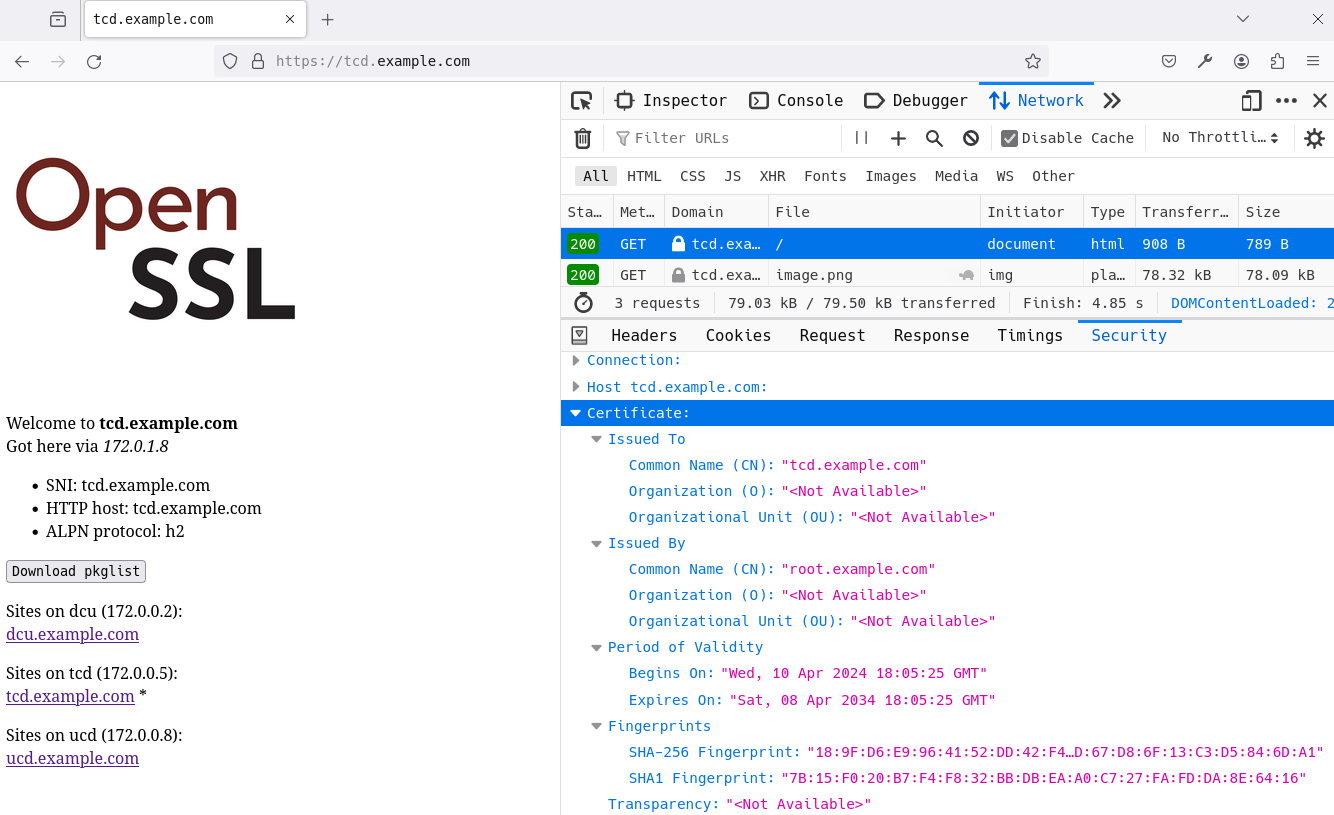
\includegraphics[width=120mm]{images/firefox.png}}
\caption[Screenshot of Mozilla Firefox when accessing tcd.example.com]{Screenshot of Mozilla Firefox when accessing tcd.example.com.}
\label{firefox_screenshot_figure}
\end{figure}

\subsection{Google Chrome}

Google Chrome is another web browser that received support for ECH in v118, October 2023. The browser was not able to use ns.example.com when set using the custom encrypted DNS option, but it was possible to work around this by setting the device's DNS resolver to ns.example.com and telling the browser to use the system resolver. Fig.~\ref{chrome_screenshot_figure} showcases the browser successfully accessing tcd.exmaple.com through 172.0.1.2, which belongs to the DCU TLS server.

\begin{figure}[ht]
\centerline{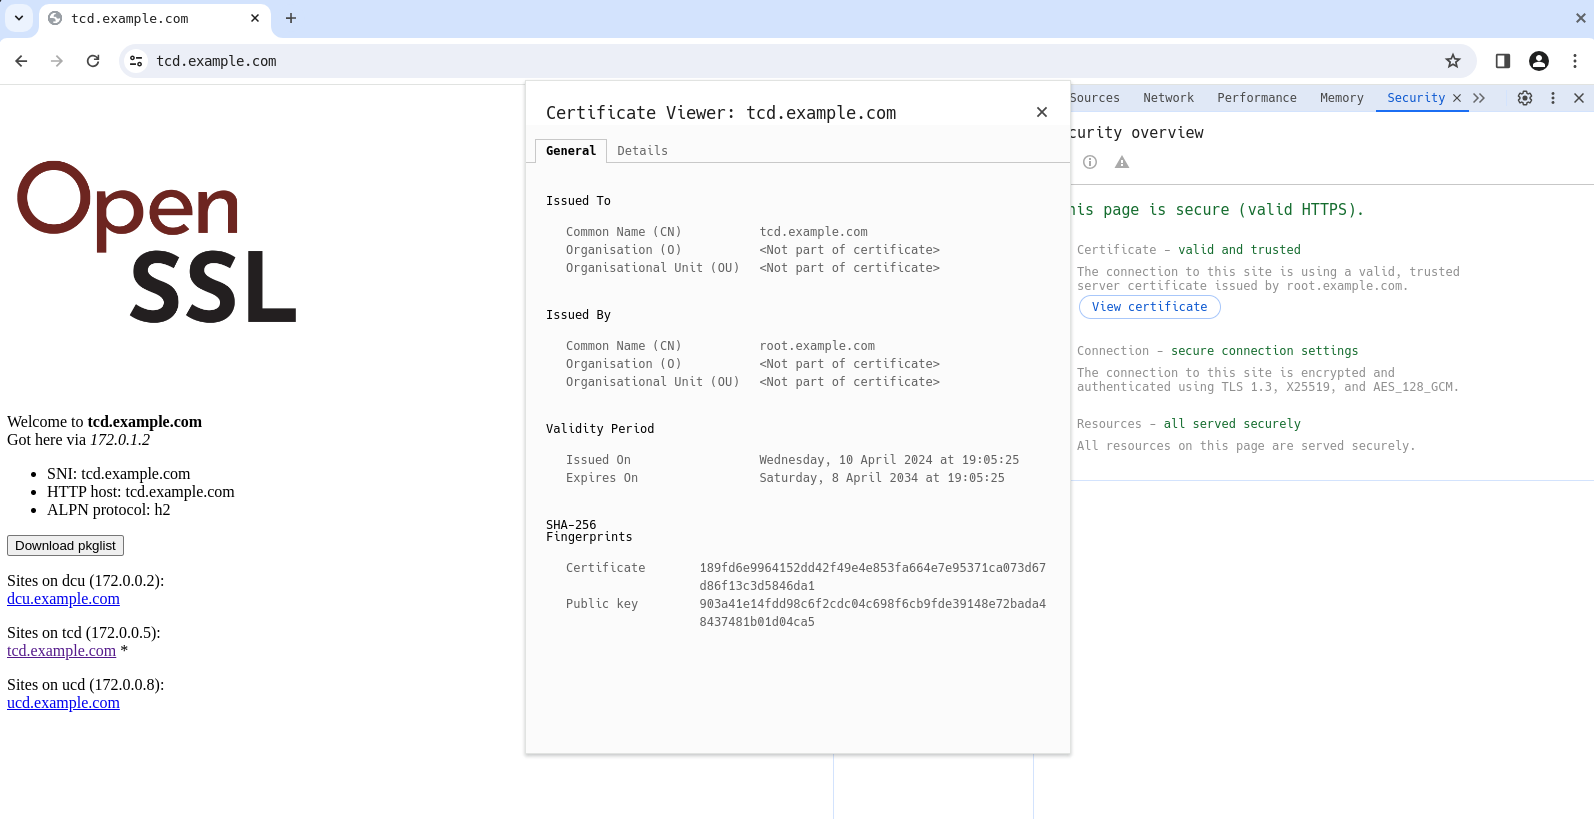
\includegraphics[width=120mm]{images/chrome.png}}
\caption[Screenshot of Google Chrome when accessing tcd.example.com]{Screenshot of Google Chrome when accessing tcd.example.com.}
\label{chrome_screenshot_figure}
\end{figure}











\section{Summary}

Virtual environments comprise of many virtual machines generated using DebVM and connected together over a bridge network. BIND9 provides authoritative name server functionality and NGINX is used as the web server on all co-operating TLS servers. WireGuard operates a VPN service to encrypt all server-server communication, while tc and tcpdump offer a proof-of-concept implementation of traffic obfuscation. Finally, curl, Mozilla Firefox and Google Chrome have been used as ECH-enabled clients to validate functioning of the ECH deployment model.
